We check each statement on synthetic data where the Helmholtz parts of the
drift are known exactly. \Cref{app:protocol} gives the protocol. All
couplings are computed in float64 and balanced to $10^{-11}$.

\paragraph{Finite-sample identities.}
On $400$ points in $\R^5$ with a generic cost:
\begin{itemize}
  \item adding a gradient flow $G$ to the cost changes the balanced
    coupling by $2\times10^{-14}$ in relative $\ell_1$ norm, and the
    row-stochastic one by $0.11$ (\cref{thm:identifiability});
  \item the cyclic part of $\log(P/P^\top)$ equals $-\tfrac2\eps\cyc(A)$ to
    a relative error of $5\times10^{-15}$, although the log-ratio also has
    a large gradient part, $31\%$ of its norm (\cref{cor:cyclic}).
\end{itemize}

\paragraph{Transport fields.}
On the flat torus $\T^2$ with a non-uniform density, we use a drift
$\omega=\rho(\nabla\phi+w)$ whose $p$-weighted decomposition is known by
construction: $\dv(p\,w)=0$. \Cref{fig:fields} shows the result for the
linear Randers cost with a global bandwidth. \Cref{cor:laplace} predicts
that the balanced chain moves along $-3\rho\,w$ and the row-stochastic chain
along $-3\rho(\nabla\phi+w)$.
\begin{itemize}
  \item \textbf{Direction.} The balanced transport has cosine $0.99$ with
    the predicted solenoidal field, and $-0.001$ with the gradient part.
    The row-stochastic transport has cosine $0.98$ with the whole drift.
    This holds at both drift strengths tested.
  \item \textbf{Magnitude.} The regression slope of measured on predicted
    transport approaches $1$ as the bandwidth shrinks (\cref{tab:sweep}).
    The deficit roughly halves when $h$ halves, as expected from an $O(h)$
    correction.
  \item \textbf{Solver check.} Computing the prediction with a finite-volume
    weighted Helmholtz solver instead of the known $w$ gives the same
    cosine and slope.
\end{itemize}

\begin{figure*}[t]
  \centering
  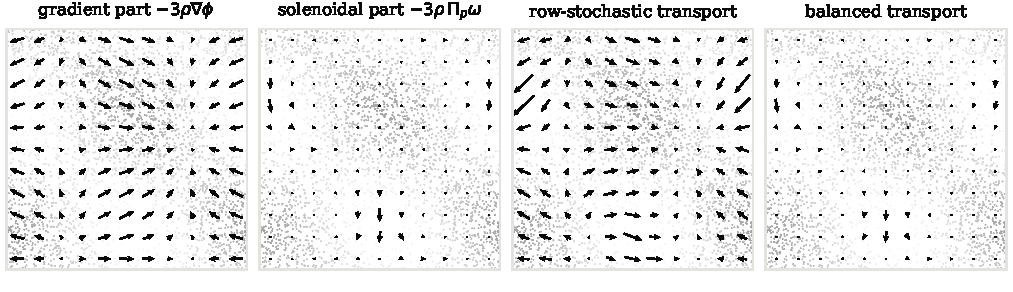
\includegraphics[width=\textwidth]{figures/torus_fields.pdf}
  \caption{Transport on the flat torus, drift $\omega=\rho(\nabla\phi+w)$
    with $\dv(p\,w)=0$, $\rho=0.3$, linear Randers cost, global bandwidth
    ($n=3000$, $h=0.04$). Arrows are averages over grid cells, all panels on
    one scale; grey dots are the samples, darker where $p$ is higher. The
    row-stochastic chain moves along the whole drift. The balanced chain
    moves along its $p$-solenoidal part only, as predicted by
    \cref{cor:laplace}.}
  \label{fig:fields}
\end{figure*}

\begin{table}[t]
  \caption{Bandwidth sweep at a fixed number of neighbours per kernel, $\rho=0.3$:
    slope of measured on predicted transport (1 is exact), and the
    gradient leak under per-row bandwidths with the cosine of its
    \cref{cor:leak} prediction.}
  \label{tab:sweep}
  \centering\small
  \begin{tabular}{@{}rrccc@{}}
    \toprule
    $h$ & $n$ & slope, Sk & slope, RS & per-row cos \\
    \midrule
    $0.070$ & $980$  & $0.69$ & $0.64$ & $0.95$ \\
    $0.050$ & $1920$ & $0.80$ & $0.78$ & $0.96$ \\
    $0.040$ & $3000$ & $0.84$ & $0.86$ & $0.96$ \\
    $0.035$ & $3918$ & $0.86$ & $0.89$ & $0.97$ \\
    \bottomrule
  \end{tabular}
\end{table}

\paragraph{Leakage.}
\Cref{fig:leak} compares a gradient drift with a solenoidal drift of the
same strength, under the three costs.
\begin{itemize}
  \item \textbf{Linear cost, global bandwidth.} The gradient drift
    produces no balanced transport, below $4\times10^{-11}$ for every
    $\rho$, at the level of the Sinkhorn tolerance
    (\cref{cor:gauge,cor:laplace}).
  \item \textbf{Linear cost, per-row bandwidth.} The gradient drift leaks
    at first order in $\rho$, and strongly: about $80\%$ of the transport
    produced by a solenoidal drift of the same strength. The leak matches
    \cref{cor:leak}(2) with cosine $0.96$ to $0.97$ and slope $0.92$. We
    obtain it from the measured per-row bandwidths through a weighted
    Helmholtz solve.
  \item \textbf{Squared cost, global bandwidth.} The leak is also linear in
    $\rho$ over the range we can simulate, at about $14\%$ of the
    transport of a solenoidal drift under the same cost. It shrinks when the sample size grows at fixed
    bandwidth ($0.020$, $0.017$, $0.013$ at $\rho=0.4$ for
    $n=980,1960,3920$, $h=0.07$), so it is at least partly a finite-sample
    effect. We do not reach the third-order regime of \cref{cor:leak}(1),
    and we leave its numerical confirmation open.
\end{itemize}

\begin{figure}[t]
  \centering
  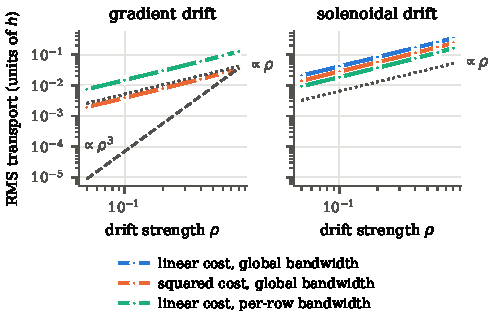
\includegraphics[width=\columnwidth]{figures/leakage.pdf}
  \caption{RMS balanced transport against drift strength on the torus
    ($n=3000$, $h=0.04$). Left: a gradient drift. With the linear cost and
    a global bandwidth it stays below $4\times10^{-11}$ for every $\rho$,
    outside the plotted range. Right: a solenoidal drift of the same
    strength, for reference.}
  \label{fig:leak}
\end{figure}
